\section{\Lib{}: Background, Design and its Motivation}
\label{s:perf}

Current deterministic execution systems \cite{liu_dthreads:_2011,merrifield_conversion:_2013,kai_lu_efficient_2014} allow an arbitrary multi-threaded program written in a conventional parallel programming language (like C or Java) to execute in a deterministic manner (the \emph{singleton} definition of determinism \cite{Lu:2011:DISC}). The program's output and succession of internal states become solely a function of the program's explicit inputs 
and are unaffected by the non-deterministic interleaving of shared memory operations or scheduler policy.

\lib{} is intended as a high-performance, deterministic, drop-in replacement library for pthreads. Any pthreads-compatible program may be linked with \lib{} to create a deterministic, yet efficient version of the same. Determinism is assured for all programs, even those with data races. However, the use of atomic instructions or ad-hoc synchronization methods such as spinning on flag variables may (deterministically) result in incorrect behavior (\S\ref{s:adhoc}). Further, in order to ensure correctness memory conflicts are merged at a byte granularity. In the presence of data races, this can result in outcomes not possible in non-deterministic execution \cite{kai_lu_efficient_2014}. In these aspects \lib{} offers the same determinism and progress guarantees as other recent deterministic execution systems \cite{liu_dthreads:_2011,kai_lu_efficient_2014}. In contrast with some prior work \cite{olszewski_kendo:_2009}, \lib{} does not assume that programs are race-free.

We now briefly summarize the design of \lib{}.
To achieve determinism, \lib{} uses a deterministic, instruction-count based logical clock (\S\ref{s:dlc}), and memory isolation using page table manipulation and deterministic, byte-level merging at synchronization points (\S\ref{s:commit}). All pthreads synchronization operations are replaced with deterministic equivalents, which ensure a strict ordering of these operations (\S\ref{s:detsync}) based on the logical clock. \lib{} also supports ad-hoc synchronization through periodically (and deterministically) synchronizing memory in the absence of explicit synchronization operations (\S\ref{s:adhoc}). 

Below, we provide background on deterministic concurrency, and describe and motivate each of the design choices made in \lib{}.

All deterministic execution schemes must provide two key components: 1) a \emph{deterministic logical clock} to enforce a deterministic order of synchronization operations and 2) a \emph{deterministic memory consistency model} that ensures loads return deterministic values even in the presence of unsynchronized accesses. Together, these two components are sufficient to guarantee the determinism of arbitrary programs. Below, we present and motivate the primary decisions that guided the design of \lib{}, while reviewing the alternative designs used in prior work.

\subsection{Deterministic Logical Clocks}
\label{s:dlc}

A deterministic logical clock is a mechanism that provides a deterministic total ordering for synchronization operations. A total order is necessary because synchronization operations must be globally coordinated in the general case when the system has no knowledge of what synchronization threads may attempt to perform next. The deterministic logical clock must ensure that, e.g., if two threads try to acquire the same lock, the same thread always wins. 

\begin{figure}
\centering
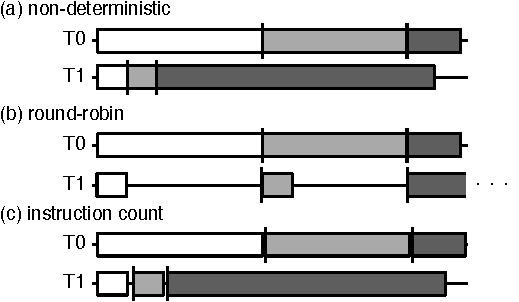
\includegraphics[width=3.0in]{figures/sync-frequency.pdf}
\caption{Effect of mismatched rate of synchronization operation. Vertical bars--sync. ops, boxes--work performed. (a) Mismatch causes no waiting with non-deterministic execution, but (b) can incur extensive waiting with round-robin deterministic logical clocks. (c) An instruction-count based logical clock \cite{olszewski_kendo:_2009} incurs waits close to those of a non-deterministic system. }
\label{f:sync-freq}
\end{figure}

The simplest logical clock is a round-robin policy and has been proven to work well in many prior schemes \cite{devietti_dmp:_2009,bergan_coredet:_2010,derek_r._hower_calvin:_2011,liu_dthreads:_2011,merrifield_conversion:_2013}. The round-robin policy works well when threads perform synchronization operations at the same rate. However, a thread that performs synchronization operations frequently can end up spending most of its time waiting for a thread that synchronizes rarely (\autoref{f:sync-freq}b).

A more efficient policy was proposed in Kendo \cite{olszewski_kendo:_2009} where the number of user instructions retired determines the deterministic ordering. The number of retired instructions may be determined using either performance counters \cite{olszewski_kendo:_2009,devietti_rcdc:_2011} or compiler instrumentation \cite{kai_lu_efficient_2014}. Under this design, a deterministic total ordering is obtained by allowing only the thread with the global minimum instruction count (GMIC) to perform a synchronization operation.

If all instructions required the same amount of time to execute, the Kendo approach would produce a very good ordering in the sense that threads would never have to wait long to perform a synchronization operation (\autoref{f:sync-freq}c). However, instruction latencies can vary greatly depending on the particular instruction being executed or non-deterministic processor state (e.g cache). Compounding this issue, the library implementations of deterministic synchronization operations can contain non-deterministic code such as system calls or acquisition of spin locks for internal purposes. To avoid non-determinism, an obvious solution is to disable the instruction counting whenever such code may be executed. Both instruction latency variance and clock disabling can lead to {\it clock skew}, where the logical clock becomes increasingly disconnected from real time.

In \lib{}, we use the retired instruction count for ordering based on hardware performance counters. Threads pass a single \emph{global token} between themselves and the token can only be acquired by the GMIC thread. We mitigate clock skew by allowing clocks to deterministically ``fast-forward'' as described in \S\ref{s:fast-forward}. While we have observed a small degree of nondeterminism in our performance counter measurements (consistent with other work \cite{4636099}) our logical clock is sound in the presence of deterministic performance counters and could also be constructed from lightweight compiler-based instruction counting \cite{kai_lu_efficient_2014}.

\subsection{Deterministic Memory Consistency}

A deterministic memory consistency model ensures that loads from shared memory always return the same value across program runs even in the presence of unsynchronized accesses, i.e., data races. While most loads are well-synchronized, and thus rendered deterministic by deterministic synchronization operations (\S\ref{s:dlc}), unsynchronized loads require additional effort. While \cite{olszewski_kendo:_2009} provides deterministic memory consistency by assuming data-race-free programs, most deterministic consistency models are built around the idea of temporarily isolating each thread in its own memory space. When threads are isolated, a multi-threaded program is effectively converted into a collection of single-threaded programs, each of which are inherently deterministic. Of course, threads must periodically be allowed to communicate with each other. The strength of the memory consistency model determines when a thread's updates, accumulated in isolation, must be made visible to other threads: stronger models require updates to be shared more frequently and more widely than weaker models. The key design decision for deterministic memory consistency is the semantics of a memory fence, the mechanism that controls how updates propagate to remote threads. We refer to the process of making updates visible as a \emph{commit} operation to distinguish it from the hardware's memory fence instructions. While commit operations are not inherently deterministic, they are rendered so by enforcing a commit ordering with a deterministic logical clock (\S\ref{s:dlc}).

\subsection{Total Store Order is Enough}

\begin{figure}
\centering
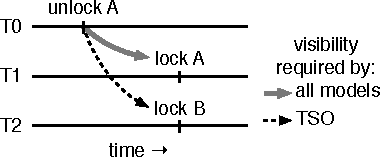
\includegraphics[width=2.7in]{figures/relaxed-consistency.pdf}
\caption{TSO requires that commits are global, while more relaxed models allow local commits that are visible to a subset of threads.}
\label{f:relaxed}
\end{figure}

Relaxing the consistency model improves the performance of determinism by making commits cheaper. Consistency models like sequential consistency and total store order require that stores become visible in a total order that all threads agree on: commits must thus be a global operation visible to all threads (\autoref{f:relaxed}). Relaxed consistency models like DRF0 \cite{devietti_rcdc:_2011} and LRC \cite{kai_lu_efficient_2014} allow commits to be ``point-to-point'' with respect to a given synchronization object, i.e., the commit performed when releasing a lock need be visible only to the thread that subsequently acquires that lock.

While an LRC-based system may in principle offer better performance than a TSO-based system, the adoption of such an extremely relaxed\footnote{It is not obvious how further relaxations beyond LRC would be possible without breaking programming language semantics.} consistency model entails several additional costs. One concern is a space leak that arises from making commits visible only via a particular synchronization object. In \cite{kai_lu_efficient_2014}, if a thread modifies some data and releases lock A, those modifications must be recorded until some other thread acquires lock A. This causes space usage to scale with the number of lock objects. In the case that no other thread ever acquires lock A, space will be permanently leaked. This space overhead is not just a theoretical concern: in \cite{kai_lu_efficient_2014} large space overheads for one LRC-based system restricted the evaluation of some programs to just four threads.

%n \S\ref{s:rfdet} we report \TODO{If we get rid of that section, just cite the RFDet paper} large space overheads for one LRC-based system, on a benchmark with only a moderate number of synchronization operations.

 In addition to its space overheads, weak consistency models like LRC are difficult for both humans \cite{adve_data_2010} and automated tools \cite{batty_mathematizing_2011,burckhardt_checkfence:_2007} to understand. LRC is more relaxed than the TSO consistency models of x86 and SPARC, and thus legacy binaries on those platforms can break when moved to LRC.

\lib{} adopts the TSO consistency model, offering a familiar programming environment and compatibility with binaries compiled for any modern hardware platform. In our evaluation (\S\ref{s:eval}), we demonstrate that efficient determinism is achievable without sacrificing TSO consistency. 

\subsection{Implementing Commits}
\label{s:commit}

While the memory consistency model does somewhat constrain the possible implementations of the commit operation, many alternative designs are still possible for a given consistency model. For instance, several deterministic execution systems implement the TSO consistency model by dividing program execution into chunks consisting of a fixed number of instructions (typically 10,000-100,000) and placing a commit at the end of each chunk \cite{bergan_coredet:_2010,derek_r._hower_calvin:_2011}. Chunks are terminated early if they contain a synchronization operation. However, memory models like TSO do not require commits at places other than synchronization operations. Thus, an even more efficient TSO-based system was proposed in \cite{liu_dthreads:_2011} where chunks are as large as the regions between synchronization operations, i.e., 
commits occur only at synchronization operations. This approach better amortizes the costs of a commit.

\begin{figure}
\centering 
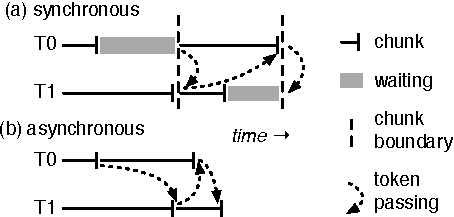
\includegraphics[width=3.0in]{figures/sync-async-chunks.pdf}
\caption{Synchronous versus asynchronous commit.}
\label{f:sync-async}
\end{figure}

Moreover, in all of these systems  \cite{bergan_coredet:_2010,derek_r._hower_calvin:_2011,liu_dthreads:_2011} commits are \emph{synchronous} operations that require coordination among all threads in the program. This synchronous approach (\autoref{f:sync-async}a) can lead to excessive waiting if threads do not naturally want to commit simultaneously.

 An alternative \emph{asynchronous} approach was proposed by \cite{merrifield_conversion:_2013}. Here, instead of a shared workspace, threads share a list of changes, and each thread applies these changes to their own workspace when appropriate. This allows threads to commit independently (\autoref{f:sync-async}b), increasing parallelism. This optimization does not break TSO because updates still appear in a total order that all threads agree on. Indeed, in modern TSO processors memory fences are implemented in a similarly asynchronous fashion.

With \lib we build upon the approach of \cite{merrifield_conversion:_2013}. However, we observe that if the number of instructions between synchronization operations is small the fixed costs of committing cannot be effectively amortized. To counteract this effect \lib{} performs adaptive coarsening of these chunks, dynamically and deterministically selecting a target chunk size to optimize performance. Coarsening does not affect TSO consistency because a fence in TSO does not require that updates be made visible immediately, merely that writes made after the fence appear no sooner than writes made before it. Coalescing multiple commits and making them visible all at once is thus valid under TSO. We provide a more detailed discussion of adaptive coarsening in \S\ref{s:optimizations}.

\subsection{Implementing Thread Isolation}
\label{s:isolation}

Many possible implementations of thread isolation have been explored by prior systems. For example, compiler instrumentation \cite{bergan_coredet:_2010, kai_lu_efficient_2014} can be used to buffer a thread's writes into per-thread store buffers. This approach introduces considerable overhead for each write and requires recompilation of all programs and libraries. Hardware store buffers \cite{devietti_rcdc:_2011,derek_r._hower_calvin:_2011,jooybar_gpudet:_2013} have also been proposed to avoid these overheads. Virtual memory protection hardware on existing systems can also be used to intercept writes on a per-page basis using the {\tt mprotect()} system call \cite{liu_dthreads:_2011} or kernel modifications \cite{merrifield_conversion:_2013}. Using virtual memory techniques requires the use of processes instead of threads.

\begin{figure}
\begin{center}
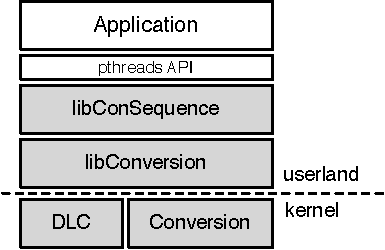
\includegraphics[width=2.2in]{figures/arch}
\caption{\lib{} architecture diagram. Shaded components indicate our system. \lib{} is implemented primarily in the form of a runtime library, but is supported by several key components implemented in the Linux kernel.}
\label{f:arch}
\end{center}
\end{figure}

%The overall architecture of \lib is shown in \autoref{f:arch}.

\lib{}'s implementation of thread isolation relies on \conversion{} \cite{merrifield_conversion:_2013}, a kernel-implemented version control system for main memory segments.
\conversion{} allows a \lib{} thread (actually a process) to operate on a {\it local copy} of a memory segment in complete isolation, until it explicitly retrieves remote changes, or commits its local changes. \lib{} provides deterministic memory consistency for only the globals and heap segments.\footnote{Shared memory segments mapped by the user will not behave deterministically.}

When a thread $T0$ begins a chunk, its globals and heap segments are updated to the latest available version of memory and each page is write-protected.  Writes will trigger a copy-on-write page fault and a reference to the new page will be stored in a thread-local dirty list. On commit, a new version is created that contains the modified pages from the dirty list. If another thread $T1$ has committed since $T0$ began its chunk, it will have to update its page table to reflect those modifications. If there is a page-level conflict (i.e., $T0$ and $T1$ wrote to the same page), a basic byte-granularity merging mechanism enforces a last-writer-wins policy. 

% \subsection{Inter-thread Communication}
% \label{s:asynchronous}

% Once a thread makes it past a synchronization point, it must retrieve any local updates and make its local changes available to other threads. 
% This may be done in one of two ways: in \cite{which}\TODO{Joe: please fill in refs}, threads execute in lock step, alternating between {\it local work} and {\it global coordination}. Under this model, all threads may make modifications directly (but in order) to a shared workspace, which forms the starting point for the next phase of {\it local work} of all threads. \TODO{Joe: is this where you used the terms centralized vs distributed before? seems quite appropriate to me now...} This \emph{synchronous} approach (\autoref{f:sync-async}a) can lead to excessive waiting as threads often execute instructions or synchronization operations at different rates.


\subsection{Deterministic Synchronization}
\label{s:detsync}

The pthreads API defines synchronization operations that are used to ensure the correctness of parallel programs. Any usable determinism system must implement a deterministic version of this API. The main primitives provided are \emph{mutual exclusion}, \emph{condition variables}, and \emph{barriers}. Additional primitives such as thread \emph{create}, \emph{join} and \emph{exit} are also typically handled by deterministic systems. Previous work has varied greatly in its support and implementation of these primitives. In \cite{liu_dthreads:_2011}, the mutual exclusion implementation replaces all locks with a single global lock. This obviously negates any performance benefits gained by fine-grained locking code.

\begin{figure}
\centering
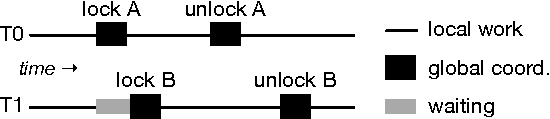
\includegraphics[width=3in]{figures/local-global}
\caption{Global coordination is required only for synchronization operations, not for critical sections.}
\label{f:local-global}
\end{figure}

\lib{} provides efficient implementations of the common pthreads synchronization primitives listed above. Each synchronization primitive is implemented using both the deterministic logical clock (\S\ref{s:dlc}) and commit (\S\ref{s:commit}) mechanisms. While highly relaxed consistency models like LRC can make commits into local operations, clock operations fundamentally require global coordination. Thus, in \lib{}, critical sections protected by different locks constitute local work that can execute concurrently, though the lock acquires and releases themselves require global coordination. In \autoref{f:local-global}, locking A and B invokes global coordination phases which must be serialized. However, between the lock and unlock operations, threads T0 and T1 can run concurrently. 

\lib{} provides the first $blocking$ implementation of a deterministic {\tt mutex\_lock()}, as opposed to the polling implementation in \cite{olszewski_kendo:_2009}. Our barrier implementation enables threads to concurrently retrieve and commit changes during the global coordination phase, a great improvement over an otherwise-serialized process. The implementation of our synchronization operations is described in detail in \S\ref{s:sync}.

\subsection{Ad Hoc Synchronization and Atomic Operations}
\label{s:adhoc}

For deterministic execution systems that perform commits at explicit synchronization operations \cite{liu_dthreads:_2011,merrifield_conversion:_2013,kai_lu_efficient_2014}, it can be difficult or impossible to support programs that communicate implicitly through shared memory. Take for example a thread $T0$ spinning on a synchronization variable $flag$ that will be set by another thread $T1$. If $T1$ commits its modification to $flag$ after $T0$'s chunk containing the ad hoc synchronization loop begins, $T0$'s chunk will never finish. This infinite loop occurs because no event will cause $T0$ to update its view of memory and see the update to $flag$ by $T1$.

One way to support this type of synchronization in \lib{} would be to set a limit on the number of instructions that can be executed within a chunk. Once that bound is hit, the thread must perform a commit operation. This would force $T0$ to break out of the spin loop and eventually see the changes made by $T1$. 

However, the choice of a per-chunk instruction limit is application specific. For some programs, termination of a chunk early can severely degrade performance. For example, we found that some benchmarks required per-chunk instruction limits to be set to 1 billion instructions to achieve equivalent performance to an execution with the limit disabled. Of course, with higher instruction limits comes higher latency of communication with ad hoc synchronization. For now, we provide this mechanism in \lib{} but we conduct our evaluation (\S\ref{s:eval}) with it disabled and leave efficient support of such programs as future work.

Atomic operations are another type of synchronization that is difficult for \lib{} to support. Because of the thread isolation we provide (\S\ref{s:isolation}), atomic writes will occur to thread-local memory and will lose the atomicity guarantees the programmer had expected. Atomic writes will be treated like any other write and are thus subject to the last-writer-wins merging policy. This can cause correctly synchronized programs to (deterministically) produce incorrect results when using \lib{}.

While \lib{} doesn't currently support atomic operations, we believe this can be easily resolved by using binary instrumentation. By replacing an atomic instruction with a \lib{} operation that acquires the token, performs the operation, and commits; we regain the atomicity.
%
%\subsection{Putting it All Together}

%\begin{figure*}
%\centering
%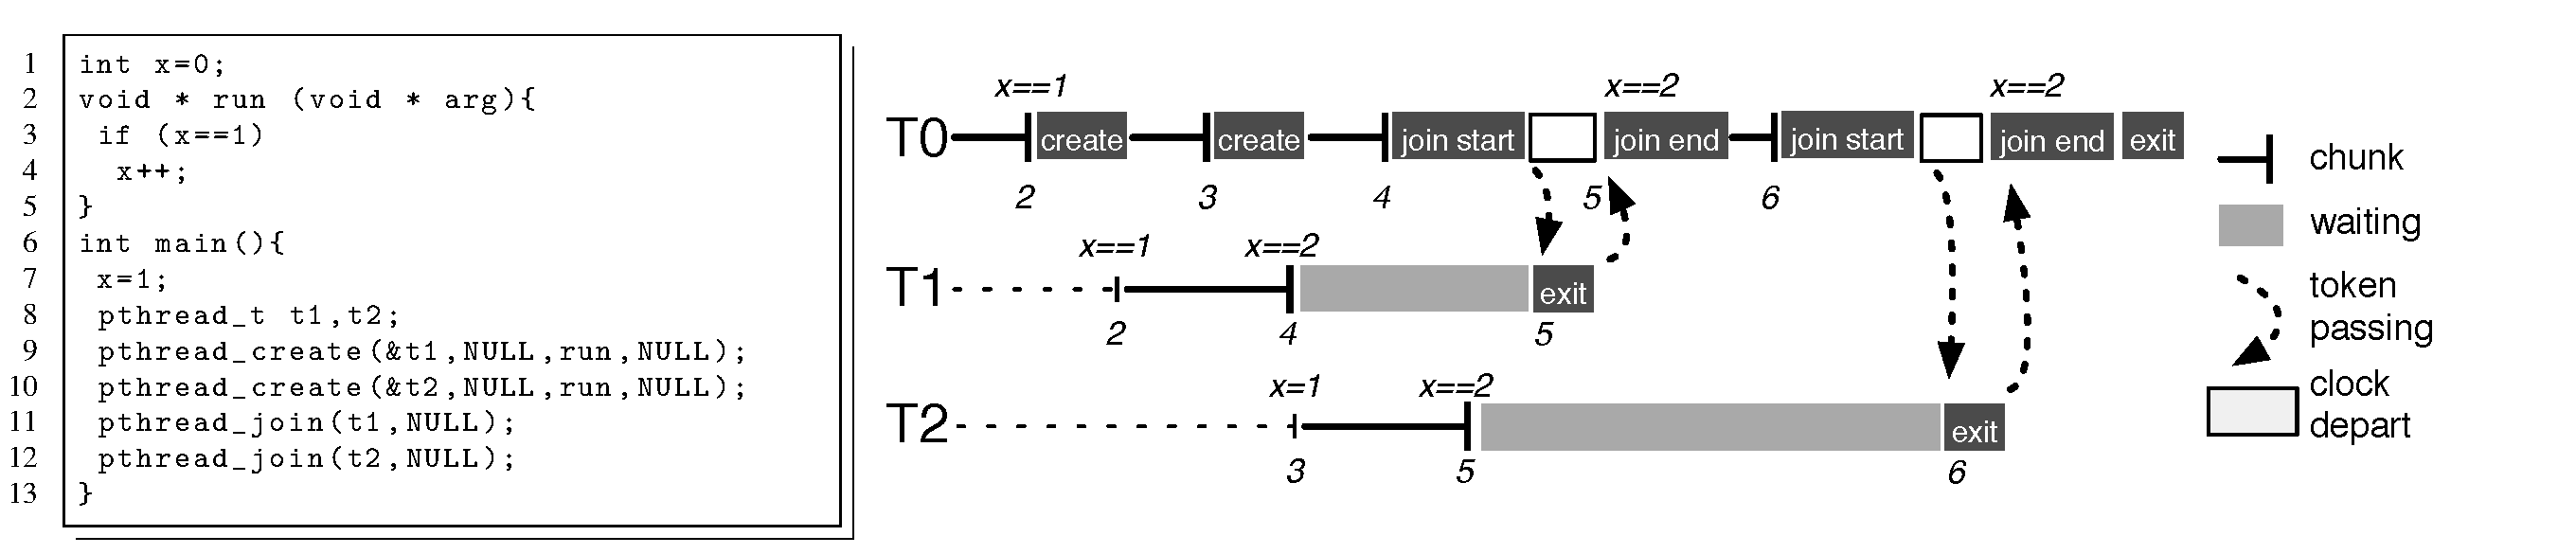
\includegraphics[width=7.25in]{figures/sample_execution}
%\caption{A deterministic execution of a simple program with \lib{}}
%\label{f:sample-execution}
%\end{figure*}

%
%Figure \ref{f:sample-execution} demonstrates the deterministic execution of a simple program using \lib{}. The initial thread T0 begins with its deterministic logical clock (shown as $DLC$) set to 0 and executes its first chunk, terminating when it invokes $pthread\_create$.

%with an equivalent operation surrounded by a pthread lock/unlock, we can regain the lost atomicity.

%\lib{} supports ad hoc synchronization by setting a bound on the number of instructions that can be executed inside a chunk. Once that bound is hit, the thread must perform a commit operation. For the example above, $t_1$ will no longer spin infinitely and will ultimately reach the bound, perform a commit and see $t_2$'s update to $flag$.  

%However, implementing this mechanism for a system with a logical clock built on hardware performance counters is not straightforward. The difficulty derives from the non-deterministic arrival of an interrupt from a counter overflow. If we set the counter to overflow after $n$ events (retired instructions), then the interrupt will arrive after $m$ events where $n \leq m \leq n+interrupt\_window$. The value of \\$interrupt\_window$ is typically informed by the size of the processor's reorder buffer.

%To avoid this non-determinism, we follow the technique introduced in \cite{tom_bergan_deterministic_2010} and set the counter to overflow after $n-interrupt\_window$ events. After receiving the interrupt, we set the processor's trap flag and single step until we reach the desired value of $n$. This ensures a deterministic commit point. Its important to note that we only perform this step when the thread begins to approach the maximum number of instructions that can be executed in a chunk.

%\subsection{Putting it all together: \Lib{} Implementation}
%
%The overall architecture of \lib is shown in \autoref{f:arch}. \lib{} is a fork of the DThreads project \cite{liu_dthreads:_2011} but reimplements the modules that perform deterministic synchronization, memory consistency and other core functionality.\footnote{We reuse the DThreads thread-local heap, shimming support and other basic infrastructure.} For programs linked with \lib{}, calls to pthreads synchronization primitives are instead handled by \lib{}.
%
%\lib{} relies on its deterministic logical clock (DLC) user space library and kernel module for deterministic synchronization. When a thread is spawned, the DLC will create a new logical clock (initialized to the parent's current clock value) and initialize the thread's performance counter to keep logical time. A thread's logical clock is updated at the following times: (a) upon completion of a chunk by reading the performance counter, (b) when a performance counter overflows or (c) when the clock is fast-forwarded (see \S\ref{s:fast-forward}). For the current GMIC thread, any clock update triggers an operation to check whether or not it is still the GMIC.  


%%% Local Variables: 
%%% mode: latex
%%% TeX-master: "paper.tex"
%%% End:
